\documentclass[italian,a4paper]{article}
\usepackage[tight,nice]{units} %unità di misura
\usepackage{babel,amsmath,amssymb,amsthm,graphicx,url}
\usepackage[text={5.5in,9in},centering]{geometry}
\usepackage[utf8x]{inputenc}
\usepackage[T1]{fontenc}
\usepackage{ae,aecompl}
\usepackage[footnotesize,bf]{caption}
\usepackage[usenames]{color}
\usepackage{textcomp}
\usepackage{gensymb}
%\include{pstricks}
\frenchspacing
\pagestyle{plain}
%------------- eliminare prime e ultime linee isolate
\clubpenalty=9999%
\widowpenalty=9999
%--- definizione numerazioni
\renewcommand{\theequation}{\thesection.\arabic{equation}}
\renewcommand{\thefigure}{\arabic{figure}}
\renewcommand{\thetable}{\arabic{table}}
\addto\captionsitalian{%
\renewcommand{\figurename}%
{Grafico}%
}
%
%------------- ridefinizione simbolo per elenchi puntati: en dash
%\renewcommand{\labelitemi}{\textbf{--}}
\renewcommand{\labelenumi}{\textbf{\arabic{enumi}.}}
\setlength{\abovecaptionskip}{\baselineskip}   % 0.5cm as an example
\setlength{\floatsep}{2\baselineskip}
\setlength{\belowcaptionskip}{\baselineskip}   % 0.5cm as an example
%--------- comandi insiemi numeri complessi, naturali, reali e altre abbreviazioni
\renewcommand{\leq}{\leqslant}
%--------- porzione dedicata ai float in una pagina:
\renewcommand{\textfraction}{0.05}
\renewcommand{\topfraction}{0.95}
\renewcommand{\bottomfraction}{0.95}
\renewcommand{\floatpagefraction}{0.35}
\setcounter{totalnumber}{5}
%---------
%
%---------
\begin{document}
\title{Relazione di laboratorio: oscilloscopio accoppiato in AC}
\author{\normalsize Ilaria Brivio (582116)\\%
\normalsize \url{brivio.ilaria@tiscali.it}%
\and %
\normalsize Matteo Abis (584206)\\ %
\normalsize \url{webmaster@latinblog.org}
\and %
\normalsize Lorenzo Rossato (579393)\\ %
\normalsize \url{supergiovane05@hotmail.com}}
\date{\today}
\maketitle
\subsection*{Stima della capacità d'ingresso}
\begin{center}
 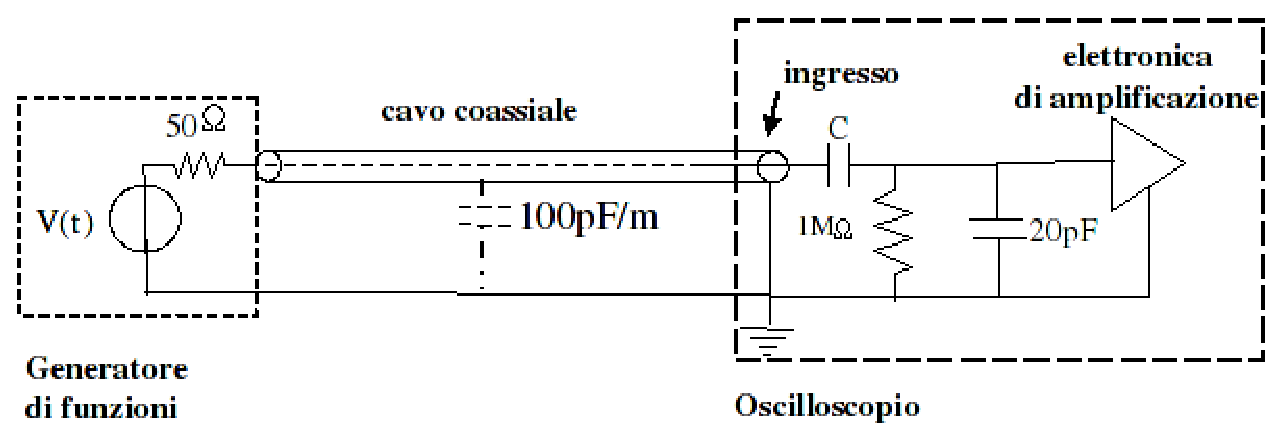
\includegraphics[height=9\baselineskip]{circuito2.eps}
\end{center}
Connettere il generatore di funzioni all’oscilloscopio mediante un cavo coassiale. Impostare il generatore di
funzioni in modo che l'uscita sia un'onda quadra di frequenza  $\unit[100]{kHz}$. Accoppiare l'oscilloscopio
in AC.
Il cavo coassiale ha una capacità di $\unitfrac[100]{pF}{m}$. Poiché $C\gg \unit[100]{pF}$, la misura della
costante di tempo ($\tau$) permette di risalire al valore di $C$. $\tau=RC$ dove $R=\unit[1]{M\ohm}$. Non è
richiesta la stima dell’errore.
\begin{align*}
    f&=\unit[1.440]{Hz} \qquad \text{onda quadra, valor medio nullo.}\\
    V_{\text{pp}}&=\unit[15]{V}\\
    V_{\text{max}}&=\unit[15.1]{V}\\
    V_{\text{max}}/e&=\unit[5.5]{V}\\
    \tau&=\unit[22.8]{ms}\\
    C=\tau /R&=\unit[22.8]{nF}\\
    f_T=\frac{1}{2 \pi RC} &=\unit[7.0]{Hz}
\end{align*}
\newpage
\subsection*{Verifica dell'utilità dell’accoppiamento AC}
Impostare il generatore di funzioni in modo che fornisca un uscita sinusoidale di ampiezza $\sim
\unit[200]{mV}$ picco-picco e valor medio $\sim \unit[5]{V}$ alla frequenza di $\unit[10]{kHz}$. Misurare
l'ampiezza del segnale in connessione DC e in connessione AC. Quale delle due modalità di misura è, a vostro
avviso, la migliore?

Non essendo possibile impostare l'ampiezza del segnale a $\unit[200]{mV}$ e ottenere l'offset richiesto,
abbiamo impostato un offset di \unit[5]{V} e un'ampiezza di circa
$\unit[800]{mV}$. In accoppiamento AC, è stato possibile misurare l'ampiezza
con divisione \unit[200]{mV}. L'ampiezza picco-picco è
risultata di \unit[832]{mV}. In accoppiamento DC, si è dovuto mantenere la
divisione a $\unit[2]{V}$ ed è risultata una misura di $\unit[800]{mV}$, ma
con errore evidentemente maggiore. La misura è stata effettuta con un segnale di frequenza \unit[10.19]{kHz}. A
frequenze più basse (si veda la frequenza di taglio sopra), il segnale viene
distorto dal condensatore inserito con l'accoppiamento AC.
\end{document}
